+In relation to the \cuda{} programming model, memory are distinguished by \textit{host} and \textit{device} memory.
In \cuda{}, the host handles allocation of device memory as well as copying from host memory to device memory and visa versa.
An example can be seen in \autoref{lst:memory-host-to-device}, where device memory is allocated, host memory copied to device memory, a kernel is launched and memory is then copied back from device to host.
\begin{lstlisting}[language=C++,caption={Example of allocation and copying from host to device},label=lst:memory-host-to-device]
int main(int argc, char ** argv) {
	unsigned char *d_in;
	cudaMalloc( &d_in, numElems * sizeof(unsigned int) )
	cudaMemcpy(d_in, h_in, numElems * sizeof(unsigned int), cudaMemcpyHostToDevice)
	example<<<blocks, threads>>>(d_in);
	cudaMemcpy(h_in, d_in, numElems * sizeof(unsigned int), cudaMemcpyDeviceToHost) }
\end{lstlisting}
Inside a kernel, a thread can access different types of device memory (local, shared and global), as described in \autoref{mortens-memory-hierarchy}.
An example of accessing local and global memory can be seen in \autoref{lst:local-global-mem-acc}.
Local memory is everything allocated in the kernel, and can be thought of a variables allocated on the "stack". In the example, a local memory access is performed every time "myId" is accessed.
Global memory can be done by accessing raw device pointers passed to the kernel, as seen in the example by accessing "d\_out" and "d\_in".
The benefit of global memory is that it can be shared across thread blocks, but it is the slowest type of device memory.
\begin{lstlisting}[language=C,caption={Local and global memory access},label=lst:local-global-mem-acc]
__global__ void local_and_global_mem(float* d_out, float* d_in){
	int myId = threadIdx.x + blockDim.x * blockIdx.x;
	d_out[myId] = d_in[myId]; }
\end{lstlisting}
Shared memory is right in between local and global memory in terms of performance, but can only be accessed within a thread block.
An example of accessing shared memory can be seen in \autoref{lst:shared-mem-acc}.
When launching a kernel that uses shared memory, the number of bytes to allocate (per block) must be specified.
This can be done by using a third argument in the kernel launch, inside "$<<< >>>$".
In the kernel, the shared memory is declared by using the keyword and "\_\_shared" (and also "extern" as it can be accessed by multiple threads).
Each thread often copies global memory to shared memory and then accesses the shared memory as much as needed before copying back to global memory.
Before starting to use the shared memory it must be ensured that all threads have copied their value from global to shared memory.
This is ensured with the synchronizer "\_\_syncthreads" (explained in details in \autoref{sec-pm-synch}).
\begin{lstlisting}[language=C,caption={Example of using shared memory},label=lst:shared-mem-acc]
__global__ void shared_mem(float * d_out, float * d_in){
	extern __shared__ unsigned int sdata[];
	int myId = threadIdx.x + blockDim.x * blockIdx.x;
	sdata[threadIdx.x] = d_in[myId];
	__syncthreads(); }
int main(int argc, char ** argv) {
	shared_mem<<< grid, threads, sizeof(unsigned int) * threads >>>( d_in, d_out ); }
\end{lstlisting}

%\autoref{fig:memory-hierarchy}
%\begin{figure}[ht]
%	\centering
%	\fbox{
%		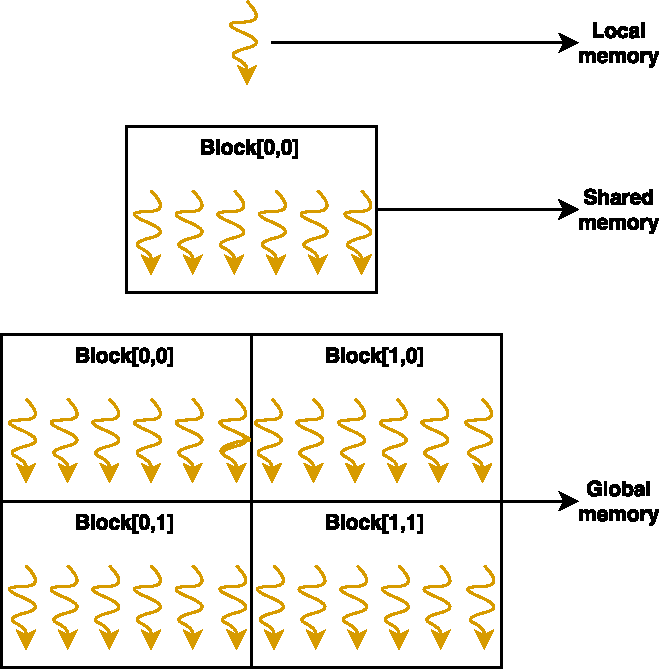
\includegraphics[width=0.6\textwidth]{figs/programming-model/memory-hierarchy.pdf}
%	}
%	\caption{Memory hierarchy}
%	\label{fig:memory-hierarchy}
%\end{figure}